\chapter{不确定性原理}
\label{chap:uncertainty-principle}

本章继续研究位置算子与动量算子之间的对易关系所产生的后果.我们主要考虑 $\mathbb R$ 上的粒子,此时
\[
[X,P]=i\hbar I.
\label{eq:uncertainty-xp-commutator}
\]
我们已经看到,对于量子谐振子的 Hamilton 算子(形如 $c_1P^2+c_2X^2$),许多分析只用到关系~\eqref{eq:uncertainty-xp-commutator}.由这一对易关系还可以推出两个主要结果:Heisenberg 不确定性原理与 Stone--von Neumann 定理.不确定性原理断言,位置的不确定度与动量的不确定度之积不可能小于 $\hbar/2$.Stone--von Neumann 定理则断言,任意满足 $[A,B]=i\hbar I$ 的自伴算子 $A,B$ 都“看起来像”作用在 $L^2(\mathbb R)$ 上的标准位置、动量算子的若干份直和.这两个结论都只在适当的技术性定义域条件下成立;我们必须认真检查这些条件.本章讨论不确定性原理,下一章讨论 Stone--von Neumann 定理.

对于满足某些定义域条件的任意 $\psi\in L^2(\mathbb R)$,不确定性原理断言
\[
(\Delta_\psi X)(\Delta_\psi P)\geq \frac{\hbar}{2},
\]
其中对任意可观测量 $A$,$\Delta_\psi A$ 表示状态 $\psi$ 下测量 $A$ 的“不确定度”(定义见定义~\ref{def:uncertainty}).这意味着,在同一个状态中,不可能同时把位置和动量的不确定度任意地变小.

只要让 $\psi$ 支持在一个很小的区间内,就可以把 $\Delta_\psi X$ 做得任意小;但这样一来,$\Delta_\psi P$ 就会很大.类似地,让动量波函数 $\widetilde\psi(p)$(见附录~\ref{app:subsec:fourier-transform})支持在一个很小的区间内,可以使 $\Delta_\psi P$ 任意小,但此时 $\Delta_\psi X$ 会变大.在位置波函数集中到单点的理想化极限中,$\psi(x)$ 会是某个 $\delta(x-a)$ 的倍数,而动量波函数则是 $e^{-ipa/\hbar}$ 的倍数;这时 $|\widetilde\psi(p)|^2$ 为常数,说明动量波函数完全铺展在整条实轴上.

不确定性原理也可以理解为:不可能同时测量量子粒子的位置和动量.根据公理~4,如果可观测量 $A$ 的谱是离散的,那么测量之后系统的状态应当立即成为 $A$ 的特征向量.如果 $A$ 的谱是连续的,则这一要求替换为:测量之后,$A$ 的不确定度应当非常小.如果能够以任意精度同时测量粒子的位置和动量,那么测量之后 $\Delta X$ 与 $\Delta P$ 都必须非常小,这将违反不确定性原理.

在日常生活的尺度上,Planck 常数很小.例如,以克、厘米、秒为质量、距离和时间的单位时,$\hbar$ 的数值为 $1.054\times10^{-27}$.因此,在能量与动量的“宏观”尺度上,位置和动量的不确定度可以同时很小;但在原子尺度上,不确定性原理会严格限制粒子的位置与动量能够局域到什么程度.

第~\ref{sec:uncertainty-first} 节将在一个看似无害的定义域假设下,证明适用于任意满足 $[A,B]=i\hbar I$ 的算子对 $A,B$ 的不确定性原理版本.第~\ref{sec:uncertainty-counterexample} 节将说明,定义域假设并没有看上去那么无害:我们会遇到两个算子,它们在 Hilbert 空间的一个稠密子空间上满足 $[A,B]=i\hbar I$,同时存在一个向量 $\psi$,使得 $A$ 的不确定度有限而 $B$ 的不确定度为零.这显然有悖于不确定性原理的精神,尽管它并不违反第~\ref{sec:uncertainty-first} 节证明的版本,因为该节定理的定义域假设对这个 $\psi$ 不成立.最后,第~\ref{sec:uncertainty-second} 节将证明,对于 $L^2(\mathbb R)$ 上通常的位置、动量算子,不会出现这样的反例:只要 $\Delta_\psi X$ 与 $\Delta_\psi P$ 都有定义,就有 $(\Delta_\psi X)(\Delta_\psi P)\geq\hbar/2$.

\section{不确定性原理的第一种形式}
\label{sec:uncertainty-first}

本节最重要的是确认:我们想要施加到向量上的每一个算子,都确实能够作用于该向量.为此,先作如下定义(与定义~\ref{def:operator-product} 相比较).

\begin{definition}[无界算子的乘积]\label{def:operator-product}
若 $A,B$ 是 $\mathcal H$ 上的无界算子,定义 $AB$ 为定义域
\[
\operatorname{Dom}(AB)=\{\psi\in\operatorname{Dom}(B)\mid B\psi\in\operatorname{Dom}(A)\}
\]
上的算子,并规定 $(AB)\psi=A(B\psi)$.
\end{definition}

即使 $\operatorname{Dom}(A)$ 与 $\operatorname{Dom}(B)$ 都在 $\mathcal H$ 中稠密,$\operatorname{Dom}(AB)$ 也可能不稠密.

回忆定义~\ref{def:uncertainty}:对称算子 $A$ 在状态 $\psi$ 下的不确定度定义为
\[
(\Delta_\psi A)^2=\left\langle\bigl(A-\langle A\rangle_\psi I\bigr)^2\right\rangle_\psi.
\label{eq:uncertainty-old}
\]
按此写法,要求 $\psi$ 属于 $(A-\langle A\rangle_\psi I)^2$ 的定义域,也就是属于 $A^2$ 的定义域.不过,由于 $A$ 对称,$\langle A\rangle_\psi=\langle\psi,A\psi\rangle$ 为实数,所以 $A-\langle A\rangle_\psi I$ 仍然是对称算子.因此,式~\eqref{eq:uncertainty-old} 可以改写为
\[
(\Delta_\psi A)^2
=\left\langle (A-\langle A\rangle_\psi I)\psi,
(A-\langle A\rangle_\psi I)\psi\right\rangle.
\]
这自然提示我们把不确定度的定义推广到只属于 $\operatorname{Dom}(A)$ 的向量.

\begin{definition}[不确定度]\label{def:uncertainty}
若 $A$ 是 $\mathcal H$ 上的对称算子,则对 $\operatorname{Dom}(A)$ 中的任意单位向量 $\psi$,定义状态 $\psi$ 下 $A$ 的不确定度 $\Delta_\psi A$ 为
\[
(\Delta_\psi A)^2
=\left\langle (A-\langle A\rangle_\psi I)\psi,
(A-\langle A\rangle_\psi I)\psi\right\rangle.
\label{eq:uncertainty}
\]
\end{definition}

展开式~\eqref{eq:uncertainty} 的右端可得
\[
(\Delta_\psi A)^2=\langle A\psi,A\psi\rangle-\bigl(\langle\psi,A\psi\rangle\bigr)^2.
\label{eq:uncertainty-expanded}
\]
这与式~\eqref{eq:uncertainty-old} 相比较.当然,如果 $\psi$ 恰好属于 $A^2$ 的定义域,定义~\ref{def:uncertainty} 与式~\eqref{eq:uncertainty-old} 一致.

\begin{proposition}[零不确定度与特征向量]\label{prop:zero-uncertainty}
若 $A$ 是 $\mathcal H$ 上的对称算子,则对 $\operatorname{Dom}(A)$ 中的任意单位向量 $\psi$,有 $\Delta_\psi A=0$ 当且仅当 $\psi$ 是 $A$ 的特征向量.
\end{proposition}

\begin{proof}
若 $\Delta_\psi A=0$,由式~\eqref{eq:uncertainty} 得
$(A-\langle A\rangle_\psi I)\psi=0$,所以 $\psi$ 是 $A$ 的特征值为 $\langle A\rangle_\psi$ 的特征向量.反之,若 $A\psi=\lambda\psi$,则
$\langle\psi,A\psi\rangle=\lambda\langle\psi,\psi\rangle=\lambda$,从而 $(A-\langle A\rangle_\psi I)\psi=0$,由式~\eqref{eq:uncertainty} 可知 $\Delta_\psi A=0$.
\end{proof}

正如本章导言所说,我们预期对可观测量 $A$ 进行测量后,系统的状态会具有很小的不确定度.若 $A$ 的谱离散,我们预期系统状态成为 $A$ 的特征向量;即使谱连续,也预期可以通过越来越精确的测量,把 $A$ 的不确定度做得任意小.现在假设希望同时观测由算子 $A,B$ 表示的两个(或更多)不同可观测量.在离散谱情形,测量后系统应当同时是 $A$ 与 $B$ 的特征向量.当 $A,B$ 对易时,这一想法是合理的:对易自伴算子有共同谱定理;在离散谱情形,这意味着它们具有由共同特征向量组成的正交归一基,并且特征值为实数(无界算子的情形仍然需要通常的对易定义域条件).

当 $A,B$ 不对易时,它们不必有共同特征向量.它们当然不可能有共同特征向量组成的正交归一基,否则它们事实上会对易.缺少共同特征向量暗示:除非两个自伴算子对易,否则不可能同时测量它们.在物理学的标准术语中,$A,B$ 被称为“不相容”的,意思是不能同时测量(代表性的一对不对易算子的共同特征向量将在练习~\ref{ex:uncertainty-joint-eigenvectors} 中分类).

在连续谱情形,特征向量的概念由相关算子具有很小不确定度的状态替代.因此,对于不对易算子,我们可能预期很难找到两个不确定度都很小的状态.下面的不确定性原理正是这一预期的严格表达.

\begin{theorem}[一般不确定性原理]\label{thm:uncertainty-general}
设 $A,B$ 是对称算子,且单位向量 $\psi$ 属于 $\operatorname{Dom}(AB)\cap\operatorname{Dom}(BA)$.则
\[
(\Delta_\psi A)^2(\Delta_\psi B)^2
\geq \frac14\left|\langle\psi,[A,B]\psi\rangle\right|^2.
\label{eq:uncertainty-general}
\]
\end{theorem}

注意,若 $\psi\in\operatorname{Dom}(AB)$,则特别有 $\psi\in\operatorname{Dom}(B)$;若 $\psi\in\operatorname{Dom}(BA)$,则 $\psi\in\operatorname{Dom}(A)$.因此,定理中的假设足以保证 $\Delta_\psi A$ 与 $\Delta_\psi B$ 能按定义~\ref{def:uncertainty} 定义.

\begin{proof}
令
\[
A'=A-\langle\psi,A\psi\rangle I,
\qquad
B'=B-\langle\psi,B\psi\rangle I.
\]
在与 $A,B$ 相同的定义域上考虑 $A',B'$;容易验证,它们仍分别在这些定义域上对称.由 Cauchy--Schwarz 不等式,
\begin{align}
\langle A'\psi,A'\psi\rangle\langle B'\psi,B'\psi\rangle
&\geq |\langle A'\psi,B'\psi\rangle|^2 \\
&\geq |\operatorname{Im}\langle A'\psi,B'\psi\rangle|^2 \\
&=\frac14\left|\langle A'\psi,B'\psi\rangle-
\langle B'\psi,A'\psi\rangle\right|^2.
\label{eq:uncertainty-cauchy}
\end{align}
定义域假设保证 $B\psi\in\operatorname{Dom}(A)$,从而 $B'\psi\in\operatorname{Dom}(A')$;交换 $A',B'$ 后同样成立.因为 $A',B'$ 对称,式~\eqref{eq:uncertainty-cauchy} 可写为
\[
\langle A'\psi,A'\psi\rangle\langle B'\psi,B'\psi\rangle
\geq \frac14\left|\langle\psi,A'B'\psi\rangle-
\langle\psi,B'A'\psi\rangle\right|^2
=\frac14\left|\langle\psi,[A',B']\psi\rangle\right|^2.
\]
恒等算子与一切算子对易,因此 $[A',B']=[A,B]$.另一方面,$\langle A'\psi,A'\psi\rangle=(\Delta_\psi A)^2$,对 $B$ 亦然.于是得到式~\eqref{eq:uncertainty-general}.
\end{proof}

令对易子为 $i\hbar I$,并对定理~\ref{thm:uncertainty-general} 两边开平方,得到如下结论.

\begin{corollary}[正则对易关系下的不确定性原理]\label{cor:uncertainty-ccr}
设对称算子 $A,B$ 在 $\operatorname{Dom}(AB)\cap\operatorname{Dom}(BA)$ 上满足
\[
[A,B]=i\hbar I.
\]
若 $\psi\in\operatorname{Dom}(AB)\cap\operatorname{Dom}(BA)$ 是单位向量,则
\[
(\Delta_\psi A)(\Delta_\psi B)\geq \frac{\hbar}{2}.
\label{eq:uncertainty-first}
\]
特别地,对 $L^2(\mathbb R)$ 中属于 $\operatorname{Dom}(XP)\cap\operatorname{Dom}(PX)$ 的任意单位向量 $\psi$,有
\[
(\Delta_\psi X)(\Delta_\psi P)\geq \frac{\hbar}{2}.
\label{eq:uncertainty-xp-first}
\]
\end{corollary}

式~\eqref{eq:uncertainty-first} 右端的 $\hbar$ 因子实质上只是 $|\langle\psi,[A,B]\psi\rangle|$.由于 $\psi$ 是单位向量且 $[A,B]=i\hbar I$,$\psi$ 从右端消失.因此,只要 $\psi$ 属于 $\operatorname{Dom}(X)\cap\operatorname{Dom}(P)$,式~\eqref{eq:uncertainty-xp-first} 两边都有意义.然而,上述证明要求 $\psi$ 同时属于 $\operatorname{Dom}(XP)$ 与 $\operatorname{Dom}(PX)$.自然的问题是:式~\eqref{eq:uncertainty-xp-first} 是否对所有 $\operatorname{Dom}(X)\cap\operatorname{Dom}(P)$ 中的 $\psi$ 成立？类似地,式~\eqref{eq:uncertainty-first} 是否对所有 $\operatorname{Dom}(A)\cap\operatorname{Dom}(B)$ 中的 $\psi$ 成立？第~\ref{sec:uncertainty-counterexample} 与~\ref{sec:uncertainty-second} 节将分别给出:第一个问题的答案是“是”,第二个问题的答案是“否”.

还可以研究使式~\eqref{eq:uncertainty-general} 取等的“最小不确定态”.

\begin{proposition}[最小不确定态的特征]\label{prop:minimum-uncertainty-general}
设 $A,B$ 对称,且单位向量 $\psi\in\operatorname{Dom}(AB)\cap\operatorname{Dom}(BA)$.式~\eqref{eq:uncertainty-general} 取等,当且仅当以下三种情况之一成立:
\begin{enumerate}
\item $\psi$ 是 $A$ 的特征向量;
\item $\psi$ 是 $B$ 的特征向量;
\item 对某个非零实数 $\gamma$,$\psi$ 是形如 $A-i\gamma B$ 的算子的特征向量.
\end{enumerate}
\end{proposition}

\begin{proof}
要在式~\eqref{eq:uncertainty-general} 中取等,式~\eqref{eq:uncertainty-cauchy} 的两步不等式都必须取等.Cauchy--Schwarz 不等式取等,当且仅当 $A'\psi=0$、$B'\psi=0$,或者对某个非零常数 $c$ 有 $A'\psi=cB'\psi$.若 $A'\psi=0$,则 $\psi$ 是特征值为 $\langle A\rangle_\psi$ 的 $A$ 的特征向量;反之,若 $\psi$ 是 $A$ 的特征向量,则 $A'\psi=0$.对 $B$ 同理.

现在设 $A'\psi,B'\psi$ 均非零,并令 $A'\psi=cB'\psi$.第二步取等当且仅当 $c=i\gamma$,其中 $\gamma\in\mathbb R\setminus\{0\}$.于是
\[
(A-\langle A\rangle_\psi I)\psi
=i\gamma(B-\langle B\rangle_\psi I)\psi,
\]
也就是
\[
(A-i\gamma B)\psi=\lambda\psi,
\qquad
\lambda=\langle A\rangle_\psi-i\gamma\langle B\rangle_\psi.
\]
反过来,若 $\psi$ 是 $A-i\gamma B$ 的特征向量,特征值写成 $\lambda=c+id$,则
\[
(c+id)\|\psi\|^2
=\langle\psi,(A-i\gamma B)\psi\rangle
=\langle\psi,A\psi\rangle-i\gamma\langle\psi,B\psi\rangle.
\]
由于 $A,B$ 对称且 $\psi$ 是单位向量,比较实部与虚部得到 $c=\langle A\rangle_\psi$、$d=-\gamma\langle B\rangle_\psi$,从而反推出上面的关系,故等号成立.
\end{proof}

\section{一个反例}
\label{sec:uncertainty-counterexample}

考虑 Hilbert 空间 $L^2([-1,1])$.作为“位置”算子,取通常的公式
\[
(A\psi)(x)=x\psi(x).
\]
由于 $x$ 限制在有界区间 $[-1,1]$ 上,$A$ 是有界算子,因此在整个 $L^2([-1,1])$ 上定义且自伴.作为“动量”算子,仍取
\[
B=-i\hbar\frac{d}{dx},
\]
其定义域取为 $[-1,1]$ 上满足周期边界条件
\[
\psi(-1)=\psi(1)
\label{eq:periodic-boundary}
\]
的连续可微函数空间.

为验证 $B$ 对称,注意对任意 $C^1$ 函数 $\phi,\psi$,分部积分给出
\[
\int_{-1}^{1}\phi(x)\frac{d\psi}{dx}(x)\,dx
=\phi(1)\psi(1)-\phi(-1)\psi(-1)
-\int_{-1}^{1}\frac{d\phi}{dx}(x)\psi(x)\,dx.
\]
若 $\phi,\psi$ 都满足周期边界条件~\eqref{eq:periodic-boundary},边界项抵消.因此 $d/dx$ 在该定义域上是反对称的,$-i\hbar d/dx$ 在该定义域上对称.事实上,函数
\[
\psi_n(x)=\frac1{\sqrt2}e^{\pi i n x},
\qquad n\in\mathbb Z,
\label{eq:periodic-eigenvectors}
\]
构成由 $B$ 的实特征值对应的特征向量组成的正交归一基;由例~\ref{ex:symmetric-orthonormal-eigenbasis},$B$ 本质自伴.

对所有 $\psi\in\operatorname{Dom}(AB)\cap\operatorname{Dom}(BA)$,直接计算得到
\[
AB\psi-BA\psi=i\hbar\psi,
\label{eq:counterexample-commutator}
\]
与通常的位置、动量算子完全一样.此外,$\operatorname{Dom}(AB)\cap\operatorname{Dom}(BA)$ 是稠密的,因为它包含所有满足 $\psi(-1)=\psi(1)=0$ 的连续可微函数.

现在取式~\eqref{eq:periodic-eigenvectors} 中的某个 $\psi_n$.显然 $\psi_n\in\operatorname{Dom}(B)$,因为 $B\psi_n$ 只是 $\psi_n$ 的倍数.由于 $\psi_n$ 是 $B$ 的特征向量,状态 $\psi_n$ 下 $B$ 的不确定度为零;另一方面,$A$ 有界,所以 $A$ 的不确定度有定义且有限.于是
\[
(\Delta_{\psi_n}A)(\Delta_{\psi_n}B)=0.
\label{eq:uncertainty-counterexample-product}
\]

式~\eqref{eq:uncertainty-counterexample-product} 怎么可能成立？这难道不是违反推论~\ref{cor:uncertainty-ccr} 中的式~\eqref{eq:uncertainty-first} 吗？答案是否定的,因为 $\psi_n$ 不满足推论的定义域假设.具体地说,$A\psi_n$ 不属于 $B$ 的定义域:$A\psi_n$ 不满足 $\operatorname{Dom}(B)$ 中的周期边界条件.因此 $\psi_n\notin\operatorname{Dom}(BA)$.

虽然这不与推论~\ref{cor:uncertainty-ccr} 矛盾,但式~\eqref{eq:uncertainty-counterexample-product} 确实违背了不确定性原理的精神.下一节将证明,对通常的位置、动量算子不会出现这种奇怪的反例.

\section{不确定性原理的第二种形式}
\label{sec:uncertainty-second}

本节将看到,当 $A,B$ 取为通常的位置、动量算子 $X,P$ 时,只要 $\Delta_\psi X$ 与 $\Delta_\psi P$ 有定义,不确定性原理就成立.我们继续使用定义~\ref{def:uncertainty},所以 $\Delta_\psi X$、$\Delta_\psi P$ 有定义只要求 $\psi\in\operatorname{Dom}(X)\cap\operatorname{Dom}(P)$.

\begin{theorem}[位置与动量的不确定性原理]\label{thm:uncertainty-strong}
设 $\psi$ 是 $L^2(\mathbb R)$ 中属于 $\operatorname{Dom}(X)\cap\operatorname{Dom}(P)$ 的单位向量,则
\[
(\Delta_\psi X)(\Delta_\psi P)\geq\frac{\hbar}{2},
\label{eq:uncertainty-strong}
\]
其中不确定度按定义~\ref{def:uncertainty} 给出.
\end{theorem}

\begin{proof}
由 Stone 定理与例~\ref{ex:translation-unitary-group},$P$ 是平移群 $U(\cdot)$ 的无穷小生成元乘以 $\hbar$.也就是说,对任意 $\psi\in\operatorname{Dom}(P)$,有
\[
(P\psi)(x)=-i\hbar\lim_{a\to0}\frac{\psi(x+a)-\psi(x)}{a},
\]
其中极限在 $L^2$ 范数意义下成立.因此
\begin{align}
\langle X\psi,P\psi\rangle
&=\lim_{a\to0}\left\langle X\psi,-i\hbar\frac{\psi(\cdot+a)-\psi}{a}\right\rangle\\
&=\lim_{a\to0}\left(\frac1a\langle x\psi(x),-i\hbar\psi(x+a)\rangle
+\frac{i\hbar}{a}\langle X\psi,\psi\rangle\right)\\
&=\lim_{a\to0}\left(\frac1a\langle i\hbar(y-a)\psi(y-a),\psi(y)\rangle
+\frac{i\hbar}{a}\langle X\psi,\psi\rangle\right),
\end{align}
最后一步作了变量代换 $y=x+a$.把积分变量改名为 $x$,得到
\begin{align}
\langle X\psi,P\psi\rangle
&=\lim_{a\to0}\left(i\hbar\left\langle\frac{\psi(x-a)-\psi(x)}a,X\psi(x)\right\rangle
+i\hbar\langle\psi(x-a),\psi(x)\rangle\right)\\
&=\langle P\psi,X\psi\rangle+i\hbar\langle\psi,\psi\rangle.
\label{eq:uncertainty-translation-identity}
\end{align}
第二个等式用到了 $X$ 的对称性,以及:若 $\psi\in\operatorname{Dom}(X)$,则对每个固定的 $a$,$\psi(x-a)\in\operatorname{Dom}(X)$.最后一个等式中,$\psi(x-a)-\psi(x)$ 带来一个负号,并使用了平移群的强连续性.

式~\eqref{eq:uncertainty-translation-identity} 正是形式上把 $X$ 移到内积右侧、使用 $XP-PX=i\hbar I$,再把 $P$ 移回左侧所得到的结果.但要使这种形式计算严格成立,必须假设 $\psi\in\operatorname{Dom}(XP)\cap\operatorname{Dom}(PX)$;式~\eqref{eq:uncertainty-translation-identity} 则只需 $\psi\in\operatorname{Dom}(X)\cap\operatorname{Dom}(P)$.

由式~\eqref{eq:uncertainty-translation-identity},对任意实数 $\alpha,\beta$,有
\[
\langle (X-\alpha I)\psi,(P-\beta I)\psi\rangle
=\langle(P-\beta I)\psi,(X-\alpha I)\psi\rangle+i\hbar\langle\psi,\psi\rangle.
\label{eq:uncertainty-shifted-inner-product}
\]
解出 $\langle\psi,\psi\rangle$,得到
\begin{align}
\langle\psi,\psi\rangle
&=\frac1{i\hbar}\left(\langle(X-\alpha I)\psi,(P-\beta I)\psi\rangle
-\langle(P-\beta I)\psi,(X-\alpha I)\psi\rangle\right)\\
&=\frac2\hbar\operatorname{Im}\langle(X-\alpha I)\psi,(P-\beta I)\psi\rangle\\
&\leq\frac2\hbar\|(X-\alpha I)\psi\|\,\|(P-\beta I)\psi\|.
\label{eq:uncertainty-strong-cauchy}
\end{align}
若 $\psi$ 是单位向量,并取 $\alpha=\langle X\rangle_\psi$、$\beta=\langle P\rangle_\psi$,则两个范数分别为 $\Delta_\psi X$ 与 $\Delta_\psi P$.于是
\[
1\leq\frac2\hbar(\Delta_\psi X)(\Delta_\psi P),
\]
这等价于式~\eqref{eq:uncertainty-strong}.
\end{proof}

第~\ref{sec:uncertainty-counterexample} 节已经说明,即使 $\operatorname{Dom}(AB)\cap\operatorname{Dom}(BA)$ 在 $\mathcal H$ 中稠密,若把 $X,P$ 换成任意满足 $AB-BA=i\hbar I$ 的无界算子,强形式也可能失败.不过,仔细观察定理~\ref{thm:uncertainty-strong} 的证明,可以看出在更一般的情形下需要哪些假设.

\begin{theorem}[半指数化对易关系下的不确定性原理]\label{thm:uncertainty-semi-exponentiated}
设 $A,B$ 是 $\mathcal H$ 上的自伴算子.假设对任意 $a\in\mathbb R$ 与 $\psi\in\operatorname{Dom}(A)$,有 $e^{iaB}\psi\in\operatorname{Dom}(A)$,并且
\[
Ae^{iaB}\psi=e^{iaB}A\psi-\hbar a e^{iaB}\psi.
\label{eq:uncertainty-semi-exponentiated}
\]
则对 $\operatorname{Dom}(A)\cap\operatorname{Dom}(B)$ 中的任意单位向量 $\psi$,有
\[
(\Delta_\psi A)(\Delta_\psi B)\geq\frac{\hbar}{2},
\]
其中不确定度按定义~\ref{def:uncertainty} 定义.
\end{theorem}

在 $\operatorname{Dom}(A)$ 上成立的关系
\[
e^{iaB}A=Ae^{iaB}+\hbar a e^{iaB},\qquad a\in\mathbb R,
\label{eq:uncertainty-semi-exponentiated-rearranged}
\]
是正则对易关系的“半指数化”形式.练习~\ref{ex:uncertainty-formal-bch} 给出一个形式论证:忽略定义域问题时,$[A,B]=i\hbar I$ 应当推出式~\eqref{eq:uncertainty-semi-exponentiated};但练习~\ref{ex:uncertainty-bch-counterexample} 说明,这种形式论证并不总能给出正确结论.第~14 章将遇到正则对易关系的“完全指数化”形式,其中 $A,B$ 都被指数化.

\begin{proof}
见练习~\ref{ex:uncertainty-prove-semi-exponentiated}.
\end{proof}

\begin{corollary}[多维位置与动量的不确定性原理]\label{cor:uncertainty-multidimensional}
对任意 $j=1,\ldots,n$,以及 $L^2(\mathbb R^n)$ 中满足 $\psi\in\operatorname{Dom}(X_j)\cap\operatorname{Dom}(P_j)$ 的单位向量 $\psi$,都有
\[
(\Delta_\psi X_j)(\Delta_\psi P_j)\geq\frac{\hbar}{2}.
\]
\end{corollary}

\begin{proof}
令 $A=X_j,B=P_j$.由第~10 章练习~\ref{ex:momentum-generates-translations},$(e^{iaB/\hbar}\psi)(x)=\psi(x+a e_j)$.于是式~\eqref{eq:uncertainty-semi-exponentiated} 成为
\[
(x_j+a)\psi(x+a e_j)=x_j\psi(x+a e_j)+a\psi(x+a e_j),
\]
显然成立.
\end{proof}

\section{最小不确定态}
\label{sec:minimum-uncertainty}

本节研究使不确定性原理取等的状态.这类状态称为最小不确定态或相干态.与命题~\ref{prop:minimum-uncertainty-general} 的一般情形一样,取等条件是一个特征向量条件.也就是说,虽然定理~\ref{thm:uncertainty-strong} 允许 $\psi$ 不属于 $\operatorname{Dom}(XP)\cap\operatorname{Dom}(PX)$,但这种放宽并不会产生新的最小不确定态.

\begin{proposition}[位置--动量最小不确定态]\label{prop:minimum-uncertainty-xp}
单位向量 $\psi\in\operatorname{Dom}(X)\cap\operatorname{Dom}(P)$ 满足
\[
(\Delta_\psi X)(\Delta_\psi P)=\frac{\hbar}{2}
\]
当且仅当存在非零实数 $\delta$ 与复数 $\lambda$,使得
\[
(X+i\delta P)\psi=\lambda\psi.
\label{eq:minimum-uncertainty-eigenvector}
\]
\end{proposition}

\begin{proof}
定理~\ref{thm:uncertainty-strong} 的证明中,除式~\eqref{eq:uncertainty-strong-cauchy} 最后一行的不等式外,所有关系都是等式.最后一行取等,当且仅当 $(X-\alpha I)\psi$ 或 $(P-\beta I)\psi$ 为零,或者 $(P-\beta I)\psi$ 是 $(X-\alpha I)\psi$ 的纯虚倍数.若 $\psi\in L^2(\mathbb R)$ 是单位向量,则 $\psi$ 与其 Fourier 变换都不可能支持在单点上,所以 $(X-\alpha I)\psi$ 与 $(P-\beta I)\psi$ 都不可能为零.因此必须有
\[
(X-\alpha I)\psi=i\gamma(P-\beta I)\psi,
\label{eq:minimum-uncertainty-shifted}
\]
其中 $\gamma\in\mathbb R\setminus\{0\}$,$\alpha=\langle X\rangle_\psi$,$\beta=\langle P\rangle_\psi$.与命题~\ref{prop:minimum-uncertainty-general} 的证明相同,式~\eqref{eq:minimum-uncertainty-shifted} 等价于 $\psi$ 是 $X-i\gamma P$ 的特征向量.令 $\delta=-\gamma$ 即得所需结论.
\end{proof}

\begin{figure}[htbp]
\centering
\includegraphics[page=265,pagebox=cropbox,trim=103.00bp 195.15bp 108.36bp 308.00bp,clip,width=0.72\textwidth]{../input/source/Quantum Theory for Mathematicians(Brian C. Hall).pdf}
\caption{满足 $\langle X\rangle=1$、$\langle P\rangle=0$ 且 $\Delta X=1/2$ 的最小不确定态.}
\label{fig:uncertainty-state-1}
\end{figure}

\begin{figure}[htbp]
\centering
\includegraphics[page=266,pagebox=cropbox,trim=91.05bp 433.44bp 100.01bp 65.16bp,clip,width=0.72\textwidth]{../input/source/Quantum Theory for Mathematicians(Brian C. Hall).pdf}
\caption{满足 $\langle X\rangle=1$、$\langle P\rangle=10$ 且 $\Delta X=1/2$ 的最小不确定态.}
\label{fig:uncertainty-state-2}
\end{figure}

\begin{proposition}[最小不确定态的显式形式]\label{prop:minimum-uncertainty-explicit}
若式~\eqref{eq:minimum-uncertainty-eigenvector} 中的参数 $\delta$ 为负,则不存在非零解.若 $\delta>0$,则对每个复数 $\lambda$,存在唯一的(相差一个常数倍意义下的)解 $\psi_{\delta,\lambda}$.它满足
\[
\langle X\rangle=\operatorname{Re}\lambda,
\qquad
\langle P\rangle=\frac{1}{\delta}\operatorname{Im}\lambda,
\qquad
\frac{\Delta X}{\Delta P}=\delta.
\]
显式地,
\[
\psi_{\delta,\lambda}(x)
=c_1\exp\left(-\frac{(x-\lambda)^2}{2\delta\hbar}\right)
=c_2\exp\left(-\frac{(x-\langle X\rangle)^2}{2\delta\hbar}\right)
\exp\left(\frac{i\langle P\rangle x}{\hbar}\right),
\label{eq:minimum-uncertainty-gaussian}
\]
其中所有期望值均在状态 $\psi_{\delta,\lambda}$ 下取.
\end{proposition}

因此,在满足 $(\Delta X)(\Delta P)=\hbar/2$ 的状态中,$\Delta X/\Delta P$ 可以是任意正实数;选定这一比值后,$\langle X\rangle$ 与 $\langle P\rangle$ 仍可任意指定为两个实数.反过来,一旦指定 $\Delta X/\Delta P$、$\langle X\rangle$ 与 $\langle P\rangle$,满足 $(\Delta X)(\Delta P)=\hbar/2$ 的量子态在相差一个整体相位的意义下是唯一的.图~\ref{fig:uncertainty-state-1}--图~\ref{fig:uncertainty-state-3} 在 $\hbar=1$ 的单位制下,绘出了若干参数对应的 $\psi_{\delta,\lambda}$ 的实部.

\begin{figure}[htbp]
\centering
\includegraphics[page=267,pagebox=cropbox,trim=90.45bp 434.40bp 99.92bp 65.59bp,clip,width=0.72\textwidth]{../input/source/Quantum Theory for Mathematicians(Brian C. Hall).pdf}
\caption{满足 $\langle X\rangle=1$、$\langle P\rangle=20$ 且 $\Delta X=1$ 的最小不确定态.}
\label{fig:uncertainty-state-3}
\end{figure}

\begin{proof}
方程 $(X+i\delta P)\psi=\lambda\psi$ 等价于
\[
x\psi+\delta\hbar\frac{d\psi}{dx}=\lambda\psi(x).
\label{eq:minimum-uncertainty-ode}
\]
这里假设 $\psi$ 属于 $P$ 的定义域,因而其分布导数是 $L^2$ 函数.若 $\psi$ 光滑,则式~\eqref{eq:minimum-uncertainty-ode} 的唯一解就是命题中给出的 $\psi_{\delta,\lambda}$;它平方可积当且仅当 $\delta>0$.即使只假设式~\eqref{eq:minimum-uncertainty-ode} 以分布意义成立,命题~\ref{prop:momentum-selfadjoint-domain} 的证明(其中以 $\exp((x-\lambda)^2/(2\delta\hbar))\psi(x)$ 替代 $e^{-x/\hbar}\psi(x)$)仍说明不存在额外解.关于 $\langle X\rangle$、$\langle P\rangle$ 与 $\Delta X/\Delta P$ 的公式,可以沿用定理~\ref{thm:uncertainty-strong} 的证明,也可以直接对式~\eqref{eq:minimum-uncertainty-gaussian} 计算.
\end{proof}

\section{练习}
\label{sec:chapter12-exercises}

\begin{exercise}[加法形式的不确定性原理]\label{ex:uncertainty-additive}
设 $\alpha>0$.证明:对 $\operatorname{Dom}(X)\cap\operatorname{Dom}(P)$ 中的任意单位向量 $\psi$,都有
\[
\alpha\Delta_\psi X+\frac1\alpha\Delta_\psi P\geq2\sqrt{\hbar}.
\]
\end{exercise}

\begin{exercise}[共同特征向量]\label{ex:uncertainty-joint-eigenvectors}
分类不对易算子 $\widehat J_1,\widehat J_2$ 的共同特征向量.设 $\widehat J_1,\widehat J_2,\widehat J_3$ 是第~\ref{sec:angular-momentum} 节在 $L^2(\mathbb R^3)$ 上定义的角动量算子.假设 $\psi$ 属于任意两个角动量算子乘积 $\widehat J_j\widehat J_k$ 的定义域(例如,$\psi$ 可以是 Schwartz 函数),并且 $\psi$ 分别是 $\widehat J_1,\widehat J_2$ 的特征值为 $\alpha,\beta$ 的特征向量.
\begin{enumerate}
\item 使用第~\ref{sec:angular-momentum} 节练习~10 的对易关系,证明 $\psi$ 是 $\widehat J_3$ 特征值为 $0$ 的特征向量.
\item 证明 $\widehat J_1,\widehat J_2$ 的特征值 $\alpha,\beta$ 必须都是零.
\item $L^2(\mathbb R^3)$ 中满足 $\widehat J_j\psi=0$($j=1,2,3$)的函数是什么类型？
\end{enumerate}
\end{exercise}

\begin{exercise}[平移与调制]\label{ex:uncertainty-translation-modulation}
给定 $\operatorname{Dom}(X)\cap\operatorname{Dom}(P)$ 中的任意单位向量 $\psi$,令
\[
\phi(x)=e^{ibx/\hbar}\psi(x-a).
\]
证明 $\phi$ 也是属于 $\operatorname{Dom}(X)\cap\operatorname{Dom}(P)$ 的单位向量,并且
\[
\langle X\rangle_\phi=\langle X\rangle_\psi+a,
\qquad \Delta_\phi X=\Delta_\psi X,
\]
以及
\[
\langle P\rangle_\phi=\langle P\rangle_\psi+b,
\qquad \Delta_\phi P=\Delta_\psi P.
\]
\end{exercise}

\begin{exercise}[相干态与降算子]\label{ex:uncertainty-coherent-states}
我们已经看到,$\psi\in\operatorname{Dom}(X)\cap\operatorname{Dom}(P)$ 是最小不确定态(即 $(\Delta_\psi X)(\Delta_\psi P)=\hbar/2$)当且仅当存在某个 $\delta>0$,使 $\psi$ 是 $X+i\delta P$ 的特征向量.此时,对任意非零常数 $c$,$\psi$ 也是 $c(X+i\delta P)$ 的特征向量.固定 $\delta>0$,定义
\[
a=\frac{1}{\sqrt{2\hbar/\delta}}(X+i\delta P).
\]
这正是质量与角频率满足 $m\omega=1/\delta$ 的谐振子的湮灭算子(见第~\ref{chap:harmonic-oscillator} 章).因此 $[a,a^*]=I$,并且存在 $L^2(\mathbb R)$ 中的特征向量链 $\psi_n$,满足定理~\ref{thm:harmonic-algebraic-structure} 中的性质.
\begin{enumerate}
\item 对任意 $\lambda\in\mathbb C$,求常数 $c_n$,使得
\[
\phi_\lambda:=\sum_{n=0}^{\infty}c_n\psi_n
\]
是 $a$ 的特征值为 $\lambda$ 的特征向量,并证明所得级数在 $\mathcal H$ 中收敛.
\item 令 $\phi_\lambda$ 为第 (a) 问得到的特征向量,并归一化使 $c_0=1$.证明
\[
\phi_\lambda=e^{\lambda a^*}\phi_0,
\qquad
e^{\lambda a^*}\phi_0:=\sum_{n=0}^{\infty}\frac{\lambda^n}{n!}(a^*)^n\phi_0,
\]
其中级数在 $L^2(\mathbb R)$ 中收敛.
\end{enumerate}
\end{exercise}

\begin{exercise}[证明半指数化关系]\label{ex:uncertainty-prove-semi-exponentiated}
沿用定理~\ref{thm:uncertainty-semi-exponentiated} 的证明思路,证明该定理.回忆第~10 章:$B/\hbar$ 是一参数酉群 $U(a):=e^{iaB/\hbar}$ 的无穷小生成元.
\end{exercise}

\begin{exercise}[形式 BCH 展开]\label{ex:uncertainty-formal-bch}
若 $X,Y$ 是有界算子,可以定义 $\operatorname{ad}_X(Y)=[X,Y]$,其中 $[X,Y]=XY-YX$.例如,$(\operatorname{ad}_X)^3(Y)=[X,[X,[X,Y]]]$.可以证明,对任意有界算子 $X,Y$,
\[
e^XYe^{-X}=e^{\operatorname{ad}_X}(Y)
=Y+[X,Y]+\frac{[X,[X,Y]]}{2!}+\frac{[X,[X,[X,Y]]]}{3!}+\cdots.
\label{eq:formal-bch}
\]
(见参考文献~\cite{Hall2013} 中的命题 2.25 与练习 2.19.)设无界自伴算子 $A,B$ 在 $\operatorname{Dom}(AB)\cap\operatorname{Dom}(BA)$ 上满足 $[A,B]=i\hbar I$.证明:如果可以令 $X=iaB/\hbar,Y=A$ 使用式~\eqref{eq:formal-bch}(尽管 $X,Y$ 无界),那么 $A,B$ 将满足式~\eqref{eq:uncertainty-semi-exponentiated}.
\end{exercise}

\begin{exercise}[无界算子中的 BCH 反例]\label{ex:uncertainty-bch-counterexample}
令 $A$ 为第~\ref{sec:uncertainty-counterexample} 节中的位置算子,令 $B$ 为该节算子的唯一自伴延拓.证明算子 $X=iaB/\hbar$ 与 $Y=A$ 不满足式~\eqref{eq:formal-bch}.

\begin{note}
这一结果说明,把有界算子的结论形式地应用于无界算子会有危险.
\end{note}

提示:先在 $B$ 的特征向量上,再推广到整个 Hilbert 空间,证明酉算子 $U(a):=\exp(iaB/\hbar)$ 表示“带绕回的平移”.
\end{exercise}
